\subsubsection{UC\theuccount-GP - Aggiunta preferenze}
		\begin{figure}[H]
			\centering
				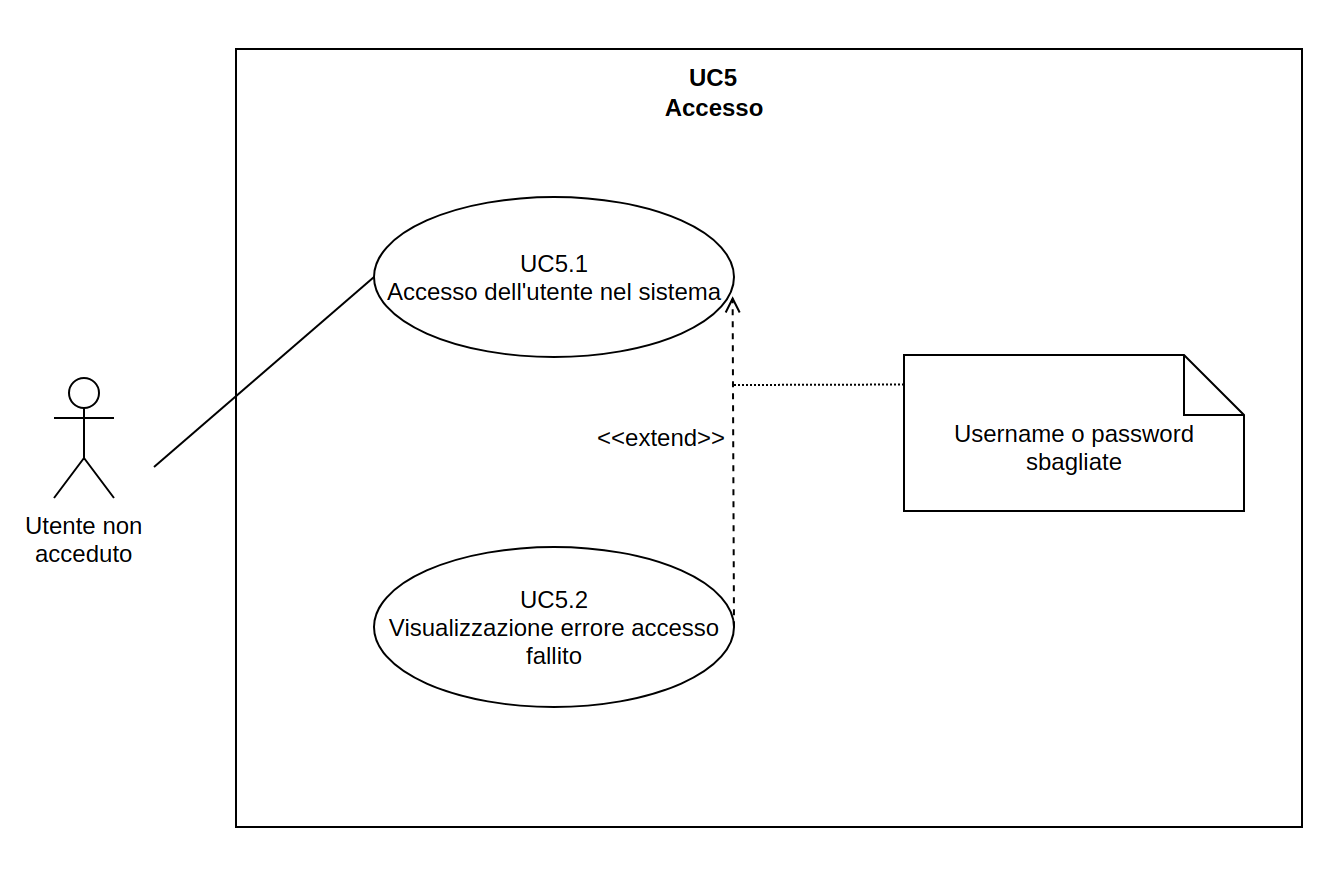
\includegraphics[width=\columnwidth]{img/UC5.png}\\
			\caption{UC\theuccount-GP - Aggiunta preferenze}
		\end{figure}
	\begin{itemize}
		\item \textbf{Codice}: UC\theuccount-GP.
		\item \textbf{Titolo}: aggiunta preferenze.
		\item \textbf{Attori primari}: utente acceduto.
		\item \textbf{Descrizione}: l’utente, date le varie opzioni per configurare Butterfly, aggiunge una
		preferenza tra Topic, giorni di calendario, piattaforma di messaggistica (Telegram o e-mail)
		preferita e la persona di fiducia che lo può sostituire.
		\item \textbf{Precondizione}: l’utente ha acceduto con le sue credenziali corrette nel sistema e non
		ha già selezionato tutte le preferenze possibili proposte da Butterfly.
		\item \textbf{Postcondizione}: la nuova configurazione contiene una o più preferenze in aggiunta rispetto a quella precedente.
		\item \textbf{Scenario Principale}:
		\begin{enumerate}
			\item Utente acceduto procede all'aggiunta di una o più preferenze.
		\end{enumerate}
	\end{itemize}


	\paragraph{UC\theuccount.1-GP - Iscrizione Topic}
		\begin{figure}[H]
			\centering
			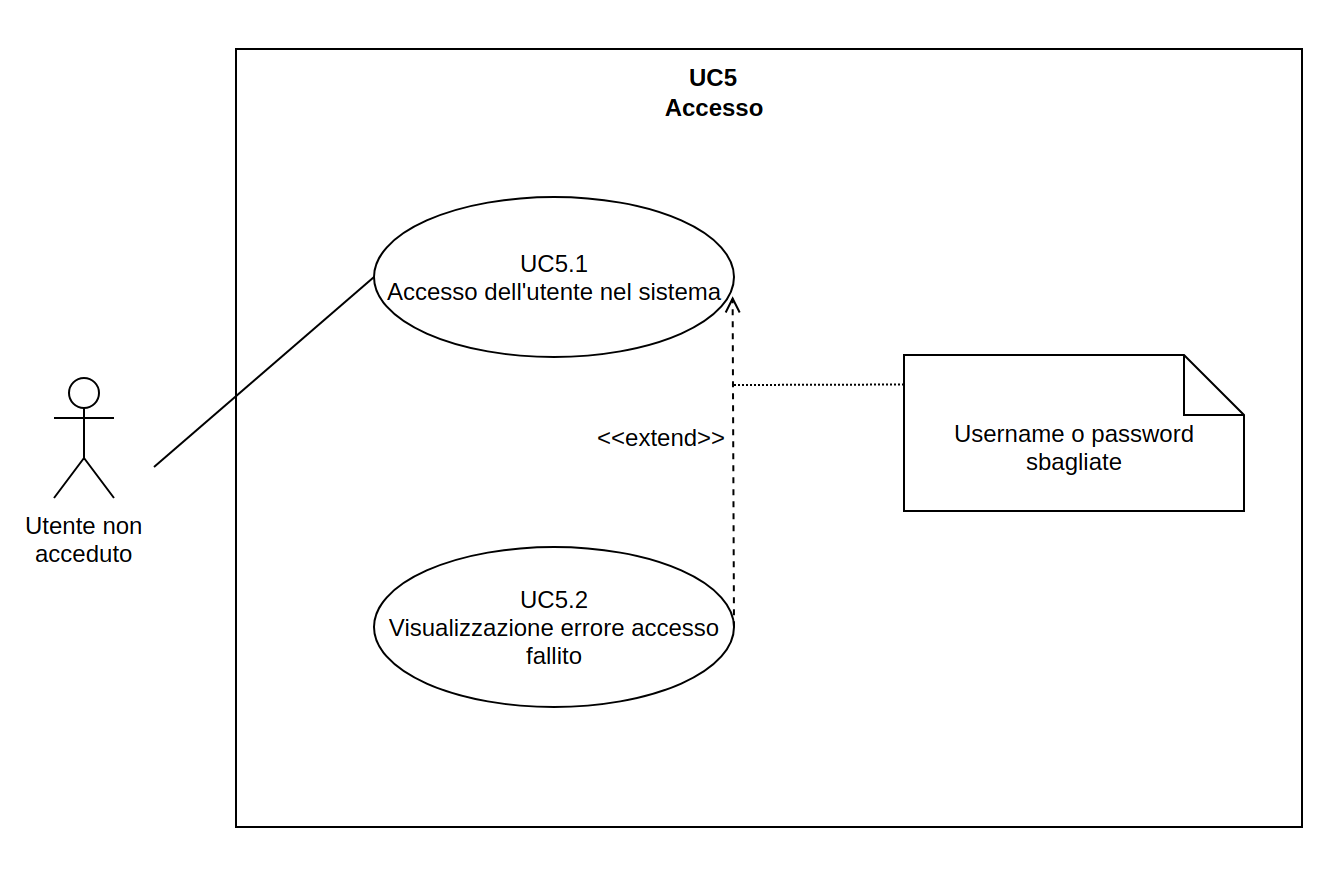
\includegraphics[width=\columnwidth]{img/UC5.png}\\
			\caption{UC\theuccount.1-GP - Iscrizione Topic}
		\end{figure}
		\begin{itemize}
			\item \textbf{Codice}: UC\theuccount.1-GP.
			\item \textbf{Titolo}: iscrizione Topic.
			\item \textbf{Attori primari}: utente acceduto.
			\item \textbf{Descrizione}: data la lista di Topic presenti, l’utente ne seleziona uno o
			più a cui è interessato, ricevendone una notifica. I Topic sono divisi per categoria e
			comprendono etichette, progetto a cui sono legate e l'applicazione di provenienza: Redmine o GitLab.
			\item \textbf{Precondizione}: l’utente ha acceduto correttamente nel sistema e non ha già
			selezionato tutti i Topic possibili proposti da Butterfly.
			\item \textbf{Postcondizione}: il numero di Topic a cui è interessato l’utente è aumentato.
			\item \textbf{Scenario Principale}:
			\begin{enumerate}
				\item Utente acceduto procede all'iscrizione di uno o più Topic.
			\end{enumerate}
		\end{itemize}
	
		\paragraph{UC\theuccount.2-GP - Aggiunta dei giorni di indisponibilità nel calendario}
			\begin{figure}[H]
				\centering
				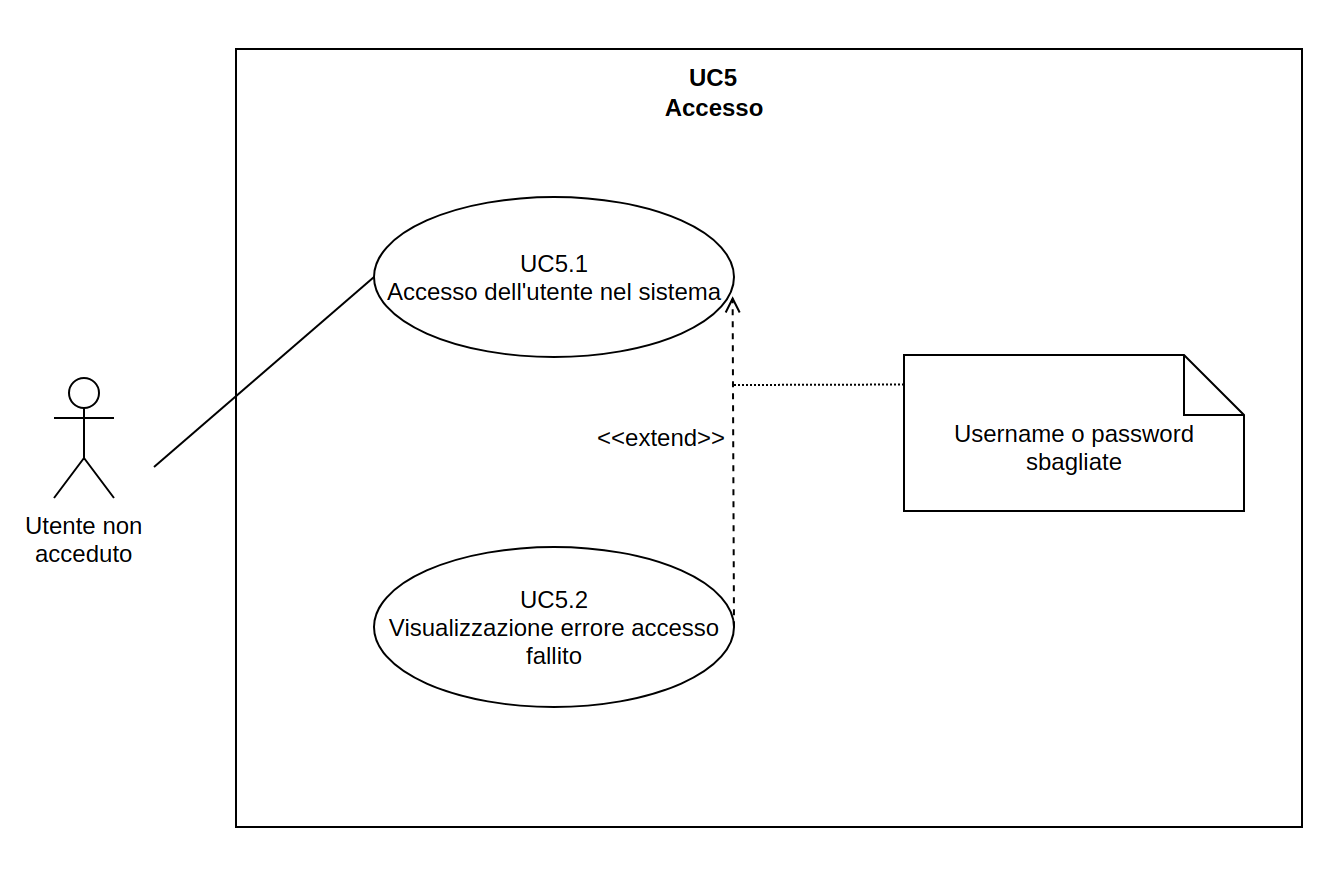
\includegraphics[width=\columnwidth]{img/UC5.png}\\
				\caption{UC\theuccount.2-GP - Aggiunta dei giorni di indisponibilità nel calendario}
			\end{figure}
			\begin{itemize}
				\item \textbf{Codice}: UC\theuccount.2-GP.
				\item \textbf{Titolo}: aggiunta dei giorni di indisponibilità nel calendario.
				\item \textbf{Attori primari}: utente acceduto.
				\item \textbf{Descrizione}: dato il calendario lavorativo, l’utente aggiunge uno o più
				giorni in cui non è reperibile e non vuole ricevere notifiche.
				\item \textbf{Precondizione}: l’utente ha acceduto correttamente nel sistema e non
				ha già selezionato tutti i giorni di indisponibilità.
				\item \textbf{Postcondizione}: il numero di giorni in cui l’utente non si rende disponibile è aumentato.
				\item \textbf{Scenario Principale}:
				\begin{enumerate}
					\item Utente acceduto procede all'inserimento di uno o più giorni di indisponibilità.
				\end{enumerate}
			\end{itemize}
		
			\paragraph{UC\theuccount.3-GP - Aggiunta della piattaforma di messaggistica preferita}
				\begin{figure}[H]
					\centering
					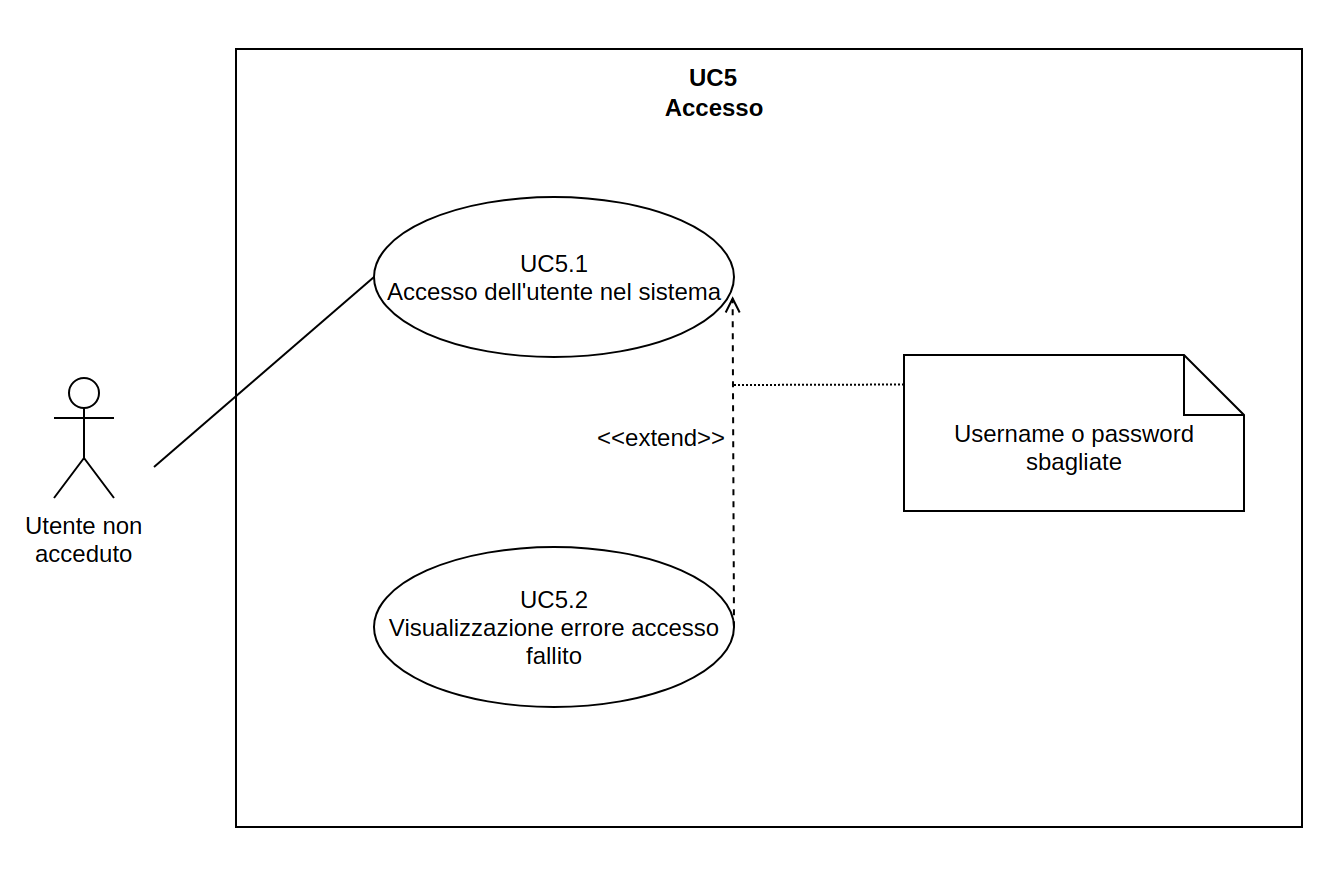
\includegraphics[width=\columnwidth]{img/UC5.png}\\
					\caption{UC\theuccount.3-GP - Aggiunta della piattaforma di messaggistica preferita}
				\end{figure}
				\begin{itemize}
					\item \textbf{Codice}: UC\theuccount.3-GP.
					\item \textbf{Titolo}: aggiunta della piattaforma di messaggistica preferita.
					\item \textbf{Attori primari}: utente acceduto.
					\item \textbf{Descrizione}: l’utente aggiunge la sua preferenza tra Telegram e email dove
					vuole ricevere le notifiche.
					\item \textbf{Precondizione}: l’utente ha acceduto correttamente nel sistema e non ha
					già selezionato tutte le piattaforme di messaggistica possibili proposte da Butterfly.
					\item \textbf{Postcondizione}: il numero di piattaforme di messaggistica selezionate dall’utente è aumentato.
					\item \textbf{Scenario Principale}:
					\begin{enumerate}
						\item Utente acceduto procede all'aggiunta di una o più piattaforme di messaggistica.
					\end{enumerate}
				\end{itemize}
			
			\paragraph{UC\theuccount.4-GP - Aggiunta persona di fiducia}
				\begin{figure}[H]
					\centering
					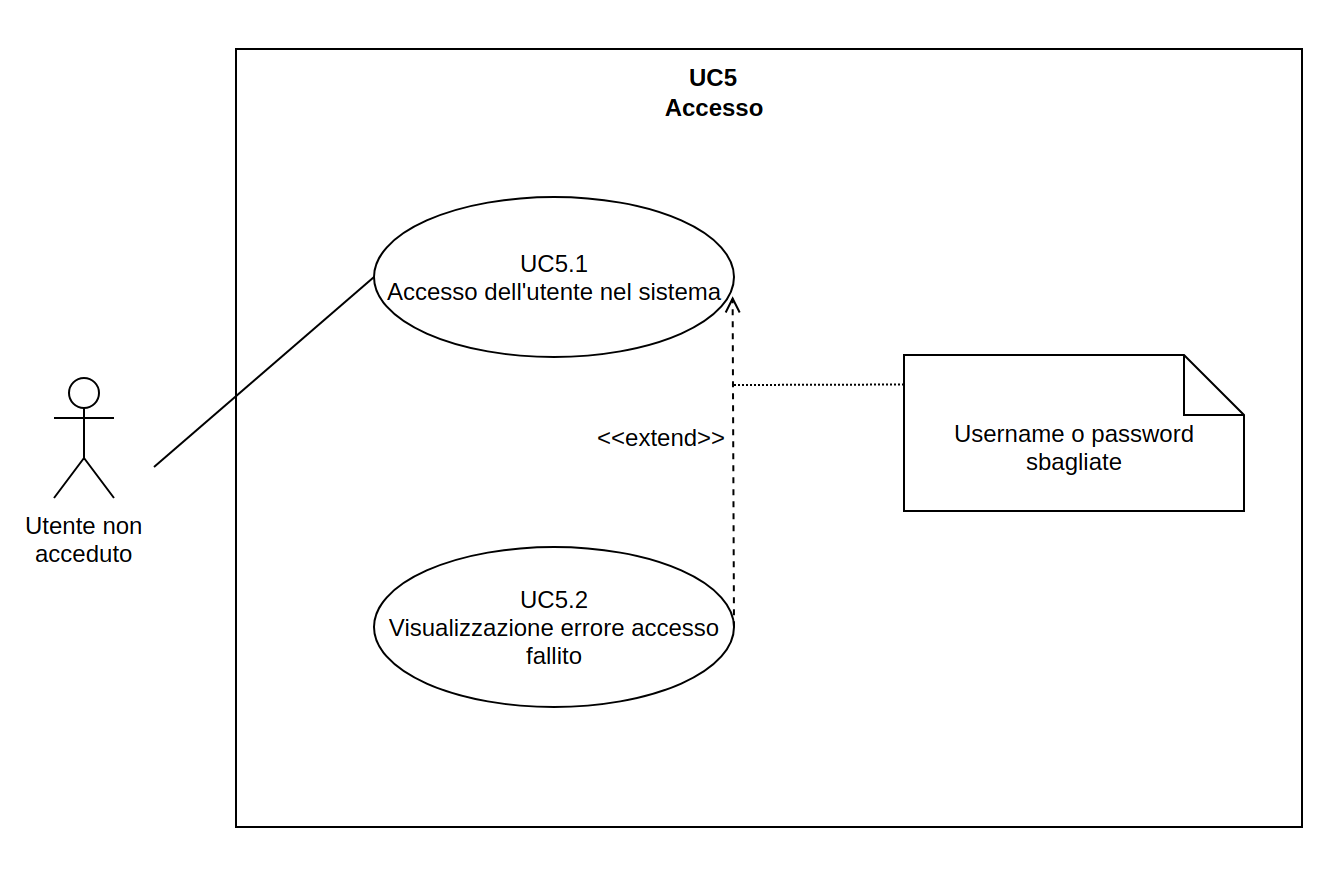
\includegraphics[width=\columnwidth]{img/UC5.png}\\
					\caption{UC\theuccount.4-GP - Aggiunta persona di fiducia}
				\end{figure}
				\begin{itemize}
					\item \textbf{Codice}: UC\theuccount.4-GP.
					\item \textbf{Titolo}: aggiunta persona di fiducia.
					\item \textbf{Attori primari}: utente acceduto.
					\item \textbf{Descrizione}: l’utente acceduto aggiunge l'utente legato a un ID di sua preferenza a
					cui inoltrare i messaggi in caso di indisponibilità.
					\item \textbf{Precondizione}: l’utente ha acceduto con le sue credenziali corrette nel
					sistema e non ha già selezionato la persona a cui inoltrare le notifiche.
					\item \textbf{Postcondizione}: la preferenza viene aggiunta correttamente.
					\item \textbf{Scenario Principale}:
					\begin{enumerate}
						\item Utente acceduto procede all'aggiunta della sua persona di fiducia.
					\end{enumerate}
					\item \textbf{Estensioni}:
					\begin{enumerate}
						\item Errore ID persona di fiducia inesistente[UC16.5-GP].
					\end{enumerate}
				\end{itemize}
			
			\paragraph{UC\theuccount.5-GP - Errore ID persona di fiducia inesistente}
				\begin{figure}[H]
					\centering
					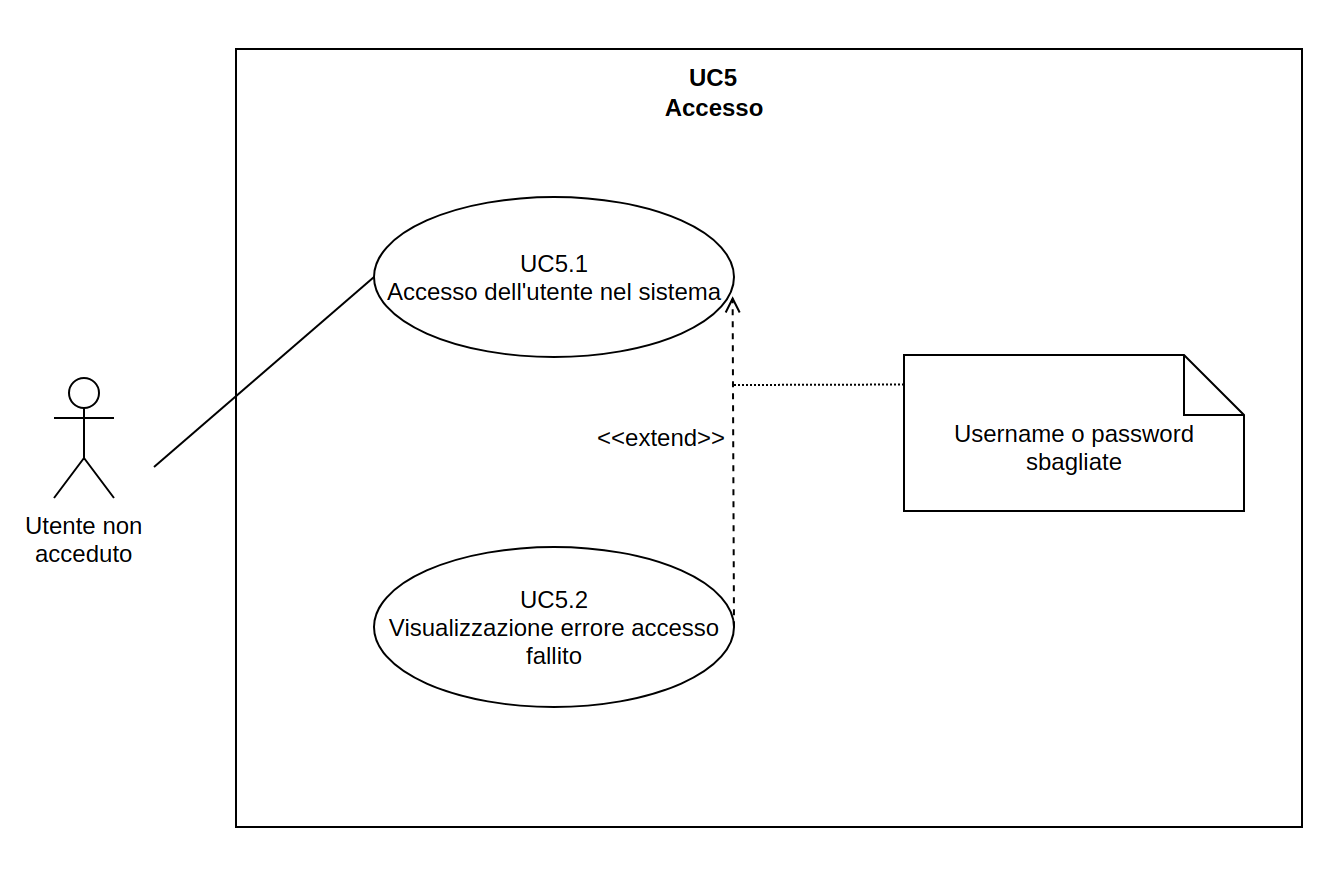
\includegraphics[width=\columnwidth]{img/UC5.png}\\
					\caption{UC\theuccount.5-GP - Errore ID persona di fiducia inesistente}
				\end{figure}
				\begin{itemize}
					\item \textbf{Codice}: UC\theuccount.5-GP.
					\item \textbf{Titolo}: errore ID persona di fiducia inesistente.
					\item \textbf{Attori primari}: utente acceduto.
					\item \textbf{Descrizione}: l’utente viene avvisato che ha inserito un ID utente errato.
					\item \textbf{Precondizione}: l’utente ha acceduto con le sue credenziali corrette nel
					sistema e non ha già selezionato la persona a cui inoltrare le notifiche.
					\item \textbf{Postcondizione}: il sistema comunica all’utilizzatore l’errore di preferenza.
					\item \textbf{Scenario Principale}:
					\begin{enumerate}
						\item Utente acceduto procede all'aggiunta della sua persona di fiducia ma questa non esiste e
						visualizza l'errore.
					\end{enumerate}
				\end{itemize}
			
			\paragraph{UC\theuccount.6-GP - Aggiunta keyword per i push di GitLab}
				\begin{figure}[H]
					\centering
					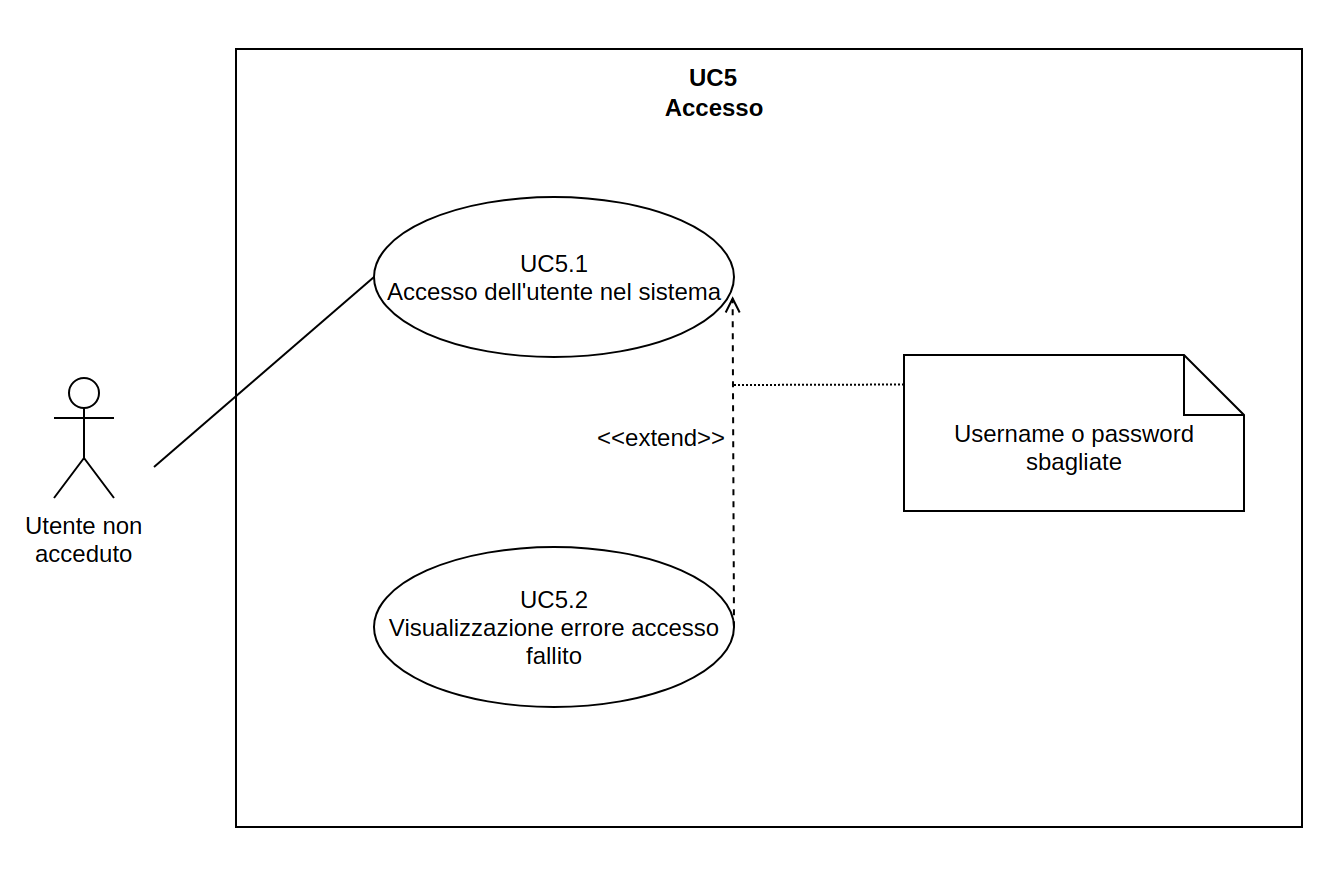
\includegraphics[width=\columnwidth]{img/UC5.png}\\
					\caption{UC\theuccount.6-GP - Aggiunta keyword per i push di GitLab}
				\end{figure}
				\begin{itemize}
					\item \textbf{Codice}: UC\theuccount.6-GP.
					\item \textbf{Titolo}: aggiunta keyword per i push di GitLab.
					\item \textbf{Attori primari}: utente acceduto.
					\item \textbf{Descrizione}: l’utente aggiunge le keyword che vuole che siano contenute
					nei messaggi di commit dei push di cui vuole ricevere la notifica.
					\item \textbf{Precondizione}: l’utente ha acceduto con le sue credenziali corrette nel sistema.
					\item \textbf{Postcondizione}: nelle nuove configurazioni dell'utente selezionato sono
					presenti una o più nuove keyword per ricevere notifiche da push di GitLab.
					\item \textbf{Scenario Principale}:
					\begin{enumerate}
						\item Utente acceduto procede all'aggiunta di una o più nuove keyword.
					\end{enumerate}
				\end{itemize}